% =============================================================================
%  System Design
% =============================================================================
\section{System Design}
\label{sec:system_design}

\subsection{Overview}

The \emph{Futoshiki VifeAgent} system is a research and demonstration platform
built around a single puzzle domain — Futoshiki — with two distinct runtime
faces: a \emph{solver benchmark harness} (CLI) and an \emph{interactive
visualisation application} (pygame GUI).
Ten solving algorithms are exposed through a single polymorphic interface,
ranging from exhaustive brute force to knowledge-based inference with FOL
and constraint propagation.

The codebase is organised as a set of \emph{layered packages} that enforce a
strict dependency direction: lower layers define domain objects; upper layers
consume them.
Figure~\ref{fig:arch} shows the package dependency graph.

\begin{figure}[h]
  \centering
  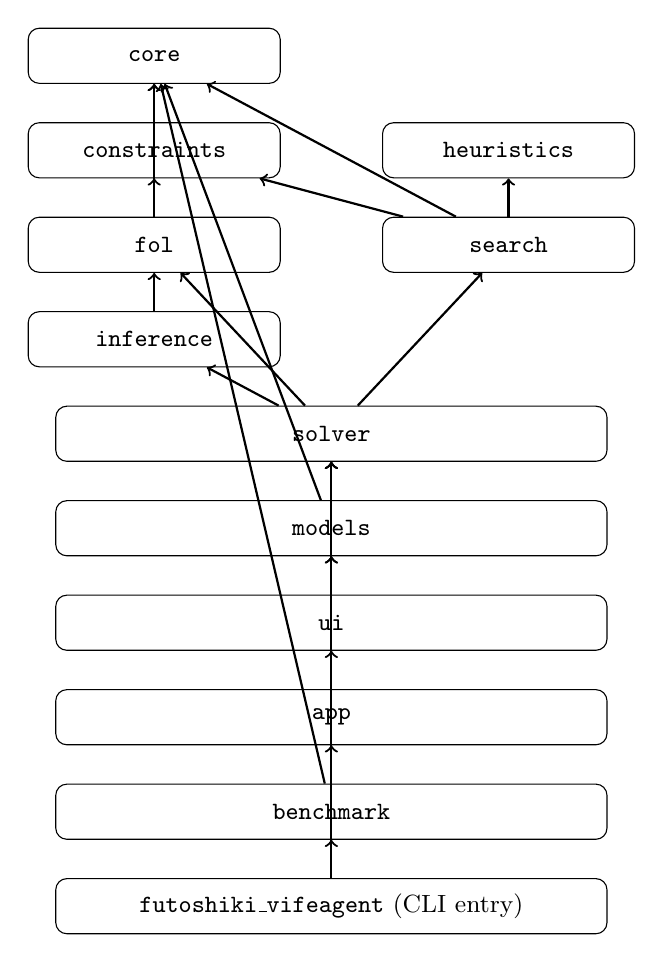
\begin{tikzpicture}[
    box/.style={draw, rounded corners, text centered, minimum width=3.2cm,
                minimum height=0.7cm, font=\small},
    arr/.style={->, thick},
    wide/.style={draw, rounded corners, text centered, minimum width=7.0cm,
                 minimum height=0.7cm, font=\small},
  ]
    % Column A (left) --------------------------------------------------------
    \node[box] (core)        at (0,0)     {\texttt{core}};
    \node[box] (constraints) at (0,-1.2)  {\texttt{constraints}};
    \node[box] (fol)         at (0,-2.4)  {\texttt{fol}};
    \node[box] (inference)   at (0,-3.6)  {\texttt{inference}};

    % Column B (right) -------------------------------------------------------
    \node[box] (heuristics)  at (4.5,-1.2) {\texttt{heuristics}};
    \node[box] (search)      at (4.5,-2.4) {\texttt{search}};

    % Spanning row -----------------------------------------------------------
    \node[wide] (solver)     at (2.25,-4.8) {\texttt{solver}};

    % Application rows -------------------------------------------------------
    \node[wide] (models)     at (2.25,-6.0) {\texttt{models}};
    \node[wide] (ui)         at (2.25,-7.2) {\texttt{ui}};
    \node[wide] (app)        at (2.25,-8.4) {\texttt{app}};
    \node[wide] (benchmark)  at (2.25,-9.6) {\texttt{benchmark}};
    \node[wide] (entry)      at (2.25,-10.8){\texttt{futoshiki\_vifeagent} (CLI entry)};

    % Arrows -----------------------------------------------------------------
    \draw[arr] (constraints) -- (core);
    \draw[arr] (fol)         -- (core);
    \draw[arr] (fol)         -- (constraints);
    \draw[arr] (inference)   -- (fol);
    \draw[arr] (search)      -- (core);
    \draw[arr] (search)      -- (constraints);
    \draw[arr] (search)      -- (heuristics);
    \draw[arr] (solver)      -- (inference);
    \draw[arr] (solver)      -- (search);
    \draw[arr] (solver)      -- (fol);
    \draw[arr] (models)      -- (solver);
    \draw[arr] (models)      -- (core);
    \draw[arr] (ui)          -- (models);
    \draw[arr] (app)         -- (ui);
    \draw[arr] (app)         -- (models);
    \draw[arr] (app)         -- (solver);
    \draw[arr] (benchmark)   -- (solver);
    \draw[arr] (benchmark)   -- (core);
    \draw[arr] (entry)       -- (app);
    \draw[arr] (entry)       -- (benchmark);
  \end{tikzpicture}
  \caption{Package dependency graph.  Arrows point from consumer to provider.}
  \label{fig:arch}
\end{figure}

The remainder of this section describes each layer in turn, bottom-up.

% =============================================================================
\subsection{Layer 1 — Core Domain (\texttt{core}, \texttt{constraints})}
\label{sec:layer_core}

\subsubsection{\texttt{core} Package}

The \texttt{core} package defines the immutable \emph{problem representation}:

\begin{description}
  \item[\texttt{Puzzle}] The central data object.
    Stores the grid dimension $N$, a NumPy integer array of shape $(N \times N)$
    (0 = empty cell, $1 \ldots N$ = given clue), and two lists of
    \texttt{InequalityConstraint} objects — one for horizontal constraints,
    one for vertical.
    Pre-computes $O(1)$ lookup maps (\texttt{\_h\_map}, \texttt{\_v\_map})
    and caches the lists of given/empty cells at construction time.
    \texttt{Puzzle.copy()} returns a deep copy with an independent grid array;
    constraints are shared (they are immutable problem data).

  \item[\texttt{Parser}] Deserialises the benchmark text format
    (size line, then $N$ grid rows, then $N$ h-constraint rows,
    then $N-1$ v-constraint rows) into a \texttt{Puzzle} instance.

  \item[\texttt{Formatter}] Serialises a \texttt{Puzzle} back to the same
    text format for output and benchmark comparison.
\end{description}

\subsubsection{\texttt{constraints} Package}

\begin{description}
  \item[\texttt{InequalityConstraint}] Records \texttt{cell1}, \texttt{cell2},
    and \texttt{direction} (\texttt{"<"} or \texttt{">"}).
    \texttt{is\_satisfied(puzzle)} reads both cell values from the grid and
    evaluates the comparison.

  \item[\texttt{RowUniquenessConstraint}, \texttt{ColUniquenessConstraint}]
    Auxiliary constraint types used by the AC-3 propagator when building arcs.

  \item[\texttt{AC3Propagator}] A standalone arc-consistency engine (Algorithm 3).
    Operates on a \texttt{dict[tuple[int,int], set[int]]} domain map.
    Encodes three relation types as bitmasks:
    \texttt{REL\_NEQ=1} (row/column uniqueness),
    \texttt{REL\_LT=2} ($<$ inequality),
    \texttt{REL\_GT=4} ($>$ inequality).
    Returns the pruned domain map on success or \texttt{None} on contradiction.
\end{description}

% =============================================================================
\subsection{Layer 2 — First-Order Logic (\texttt{fol})}
\label{sec:layer_fol}

The \texttt{fol} package is the project's largest layer.
It encodes the Futoshiki rules as formal logic, builds knowledge bases, and
performs logical inference.

\subsubsection{Predicates and Literals}

\texttt{predicates.py} defines the vocabulary of the logical language.
Each predicate class (\texttt{Val}, \texttt{NotVal}, \texttt{Given},
\texttt{LessH}, \texttt{GreaterH}, \texttt{Less}, \texttt{Geq}, \texttt{Diff},
\texttt{Domain}, \texttt{ValidVal}) is a frozen dataclass whose
\texttt{sign} attribute distinguishes positive (\texttt{+1}) from negative
(\texttt{-1}) literals.
The \texttt{Literal} base class provides equality, hashing, and a
\texttt{negate()} method.

\subsubsection{Axiom Schemas}

\texttt{axioms.py} contains 16 static methods (A1–A16) that take a puzzle
and emit ground clause lists.
Each axiom formalises one aspect of the Futoshiki rules — uniqueness, given
values, inequality constraints, domain definition — as described in
Section~\ref{sec:cnf_formulation}.

\subsubsection{Knowledge Bases}

Two distinct knowledge-base types are provided:

\begin{description}
  \item[\texttt{CNFClauseKnowledgeBase} (\texttt{kb.py})]
    Stores lists of clauses (each a list of \texttt{Literal} objects).
    \texttt{add\_clause()} auto-populates a \texttt{facts} set with unit
    clauses.
    Built by \texttt{CNFGenerator.generate(puzzle)}, which calls all 16 axioms
    in order.

  \item[\texttt{HornClauseKnowledgeBase} (\texttt{horn\_kb.py})]
    Stores \texttt{HornClause} objects (head + body list).
    Indexes clauses by head predicate type for $O(1)$ lookup during SLD
    resolution.
    Built by \texttt{HornClauseGenerator} (for backward chaining) or
    \texttt{HornClauseGenerator2} (for forward chaining).
\end{description}

\subsubsection{Horn Clause Generators}

\begin{description}
  \item[\texttt{HornClauseGenerator}] Implements the generate-and-test SLD
    strategy.
    Runs a four-level domain-pruning pipeline
    (exclusion $\to$ relative-size $\to$ hidden-single $\to$ AC-3)
    to narrow cell domains, then emits one \texttt{Solution} rule whose body
    chains \texttt{Domain\_r\_c} generator literals with \texttt{Diff}/\texttt{Less}
    test literals.

  \item[\texttt{HornClauseGenerator2}] Emits deductive-only Horn rules for
    forward chaining: \texttt{Given$\to$Val}, \texttt{Val+Diff$\to$NotVal},
    \texttt{LessH+Val+Geq$\to$NotVal}, etc.
    Used by \texttt{ForwardChaining} and \texttt{BacktrackingForwardChaining}.
\end{description}

\subsubsection{Unifier}

\texttt{unifier.py} implements Robinson's MGU algorithm.
See Section~\ref{sec:unification} for full details.
Three entry points are provided: \texttt{unify()} (general),
\texttt{match()} (SLD same-sign), and \texttt{resolve()} (propositional
opposite-sign).

% =============================================================================
\subsection{Layer 3 — Inference Engines (\texttt{inference})}
\label{sec:layer_inference}

\begin{description}
  \item[\texttt{ForwardChainingEngine}] Implements a fix-point
    Modus Ponens loop.
    On each iteration it scans all Horn rules and tries to match the
    body against the current fact set via \texttt{Unifier.match()}.
    Returns when no new fact can be derived.

  \item[\texttt{BackwardChainingEngine}] Implements SLD resolution as a
    Python generator.
    \texttt{\_sld\_resolve(goals, kb, theta)} selects the leftmost goal,
    indexes the KB by head, standardises-apart each candidate clause
    (renames variables with a monotonic suffix), unifies, and recursively
    resolves the new goal list.
    Backtracking is achieved by Python's built-in generator protocol —
    each \texttt{yield} is a solved substitution; the caller advances the
    generator to request the next solution.
\end{description}

These engines are \emph{pure inference components}: they know nothing about
Futoshiki specifically.
The solver layer (Section~\ref{sec:layer_solver}) is responsible for
constructing the appropriate KB and formulating the goal query.

% =============================================================================
\subsection{Layer 4 — Heuristics (\texttt{heuristics})}
\label{sec:layer_heuristics}

All heuristics implement \texttt{BaseHeuristic.estimate(state, puzzle) -> int}:

\begin{table}[h]
  \centering
  \caption{A* heuristic functions.}
  \label{tab:heuristics}
  \begin{tabular}{lll}
    \toprule
    Key & Class & Formula \\
    \midrule
    h1 & \texttt{EmptyCellHeuristic}    & Number of empty cells \\
    h2 & \texttt{DomainSizeHeuristic}   & $\sum_{(i,j)} (|\text{domain}_{ij}| - 1)$ \\
    h3 & \texttt{MinConflictsHeuristic} & Number of violated constraints \\
    h4 & \texttt{AC3Heuristic}          & h2 on AC-3-pruned domains \\
    \bottomrule
  \end{tabular}
\end{table}

h1 and h2 are admissible.
h3 counts current violations (g-function, not a true future estimate) —
used experimentally.
h4 is the most informed: it runs a full AC-3 pass on a domain copy before
evaluating h2; if AC-3 detects a contradiction, it returns a large penalty
($N^3$) to steer the search away immediately.

% =============================================================================
\subsection{Layer 5 — Search Engine (\texttt{search})}
\label{sec:layer_search}

\begin{description}
  \item[\texttt{SearchState}] An immutable snapshot of the search:
    a NumPy grid, a domain map, $g$-cost (violations so far), and the
    $f$-cost ($g + h$) used for heap ordering.

  \item[\texttt{AStarEngine}] Best-first graph search.
    Maintains a min-heap (open set) and a hash-based closed set.
    Cell selection uses MRV (Minimum Remaining Values): always expands the
    unassigned cell with the fewest legal values first, cutting the
    branching factor early.
    After assigning a value, basic singleton-fill propagation runs (or full
    AC-3 if a propagator is attached).
    The optional \texttt{on\_step} callback is invoked after each expansion
    to drive live visualisation.
\end{description}

% =============================================================================
\subsection{Layer 6 — Solver Façade (\texttt{solver})}
\label{sec:layer_solver}

\subsubsection{Abstract Base}

\texttt{BaseSolver} defines the single public contract:
\begin{lstlisting}[language=Python]
def solve(puzzle: Puzzle, on_step=None) -> tuple[Puzzle | None, Stats]
\end{lstlisting}
All solvers return a \texttt{Stats} dataclass with fields:
\texttt{time\_ms}, \texttt{memory\_kb}, \texttt{inference\_count},
\texttt{node\_expansions}, \texttt{backtracks}, \texttt{completion\_ratio}.

\subsubsection{Solver Inventory}

Ten concrete solvers are registered by the \texttt{solver\_registry}:

\begin{table}[h]
  \centering
  \caption{Solver inventory.}
  \label{tab:solvers}
  \begin{tabular}{lll}
    \toprule
    Key & Class & Core mechanism \\
    \midrule
    \texttt{brute\_force}           & \texttt{BruteForceSolver}               & Cartesian-product enumeration \\
    \texttt{forward\_chaining}      & \texttt{ForwardChaining}                & FC engine + hidden-single promotion \\
    \texttt{btfc}                   & \texttt{BacktrackingForwardChaining}    & FC + backtracking search \\
    \texttt{backward\_chaining}     & \texttt{BackwardChaining}               & Generate-and-test SLD \\
    \texttt{forward\_then\_backward}& \texttt{ForwardThenBackwardChaining}    & FC pipeline then SLD fallback \\
    \texttt{astar\_h1}              & \texttt{AStarSolver(h1)}                & A* with empty-cell count heuristic \\
    \texttt{astar\_h2}              & \texttt{AStarSolver(h2)}                & A* with domain-sum heuristic \\
    \texttt{astar\_h3}              & \texttt{AStarSolver(h3)}                & A* with min-conflicts heuristic \\
    \texttt{astar\_h4}              & \texttt{AStarSolver(h4)}                & A* with AC-3 heuristic \\
    \bottomrule
  \end{tabular}
\end{table}

\texttt{AStarSolver} is a thin wrapper: it constructs an \texttt{AStarEngine}
with the injected heuristic, calls \texttt{engine.solve()}, and wraps the
result as a \texttt{Puzzle}.
The other solvers perform their own KB construction, call the respective
inference engine, and extract the solution from the returned substitution.

% =============================================================================
\subsection{Layer 7 — Benchmark Harness (\texttt{benchmark})}
\label{sec:layer_benchmark}

\subsubsection{Puzzle Corpus}

24 benchmark puzzles are generated deterministically by \texttt{FutoshikiGenerator}
(sizes $4 \times 4$ to $9 \times 9$, four difficulty levels each).
The generator uses backtracking with MRV to fill a complete solution, then
adds inequality constraints at a configurable density, then removes given
cells while checking uniqueness via a Z3 SMT solver.
Input/expected file pairs are stored under \texttt{resource/benchmark/}.

\subsubsection{Benchmark Runner}

\texttt{benchmark.py} loads every input file, instantiates the selected solver,
calls \texttt{solver.solve()}, compares the result against the expected solution,
and records a \texttt{BenchmarkRow} to a CSV file.
The \texttt{--solver} flag selects the algorithm; \texttt{--max-n} filters by
grid size.

\subsubsection{Visualiser}

\texttt{visualize.py} reads the CSV outputs and produces:
\begin{itemize}
  \item Line charts of time, memory, node expansions, and backtracks by puzzle size.
  \item A completion-ratio heatmap (solver × puzzle).
  \item Optionally, \LaTeX\ table fragments for inclusion in reports.
\end{itemize}

% =============================================================================
\subsection{Layer 8 — Application Layer (\texttt{app}, \texttt{models}, \texttt{ui})}
\label{sec:layer_app}

\subsubsection{State Machine (\texttt{models})}

The application operates in three modes captured by the \texttt{AppMode} enum:

\begin{description}
  \item[\texttt{KB}] CNF knowledge-base viewer.
    Displays the clause list generated from the active puzzle; supports hover
    and click-to-explain interactions.
  \item[\texttt{PLAY}] Manual interaction.
    The user selects cells, enters values, toggles pencil marks, requests hints,
    and undoes edits.
  \item[\texttt{SOLVE}] Step-by-step solver visualisation.
    A background thread runs the selected solver; the main loop drains a
    \texttt{queue.Queue[SolveStep]} and animates each node expansion.
\end{description}

\texttt{GameState} is a flat dataclass that holds \emph{all} mutable
application state — mode, active board, CNF KB, solver thread handle,
step queue, backtrack flash timers, shake animation timers, notification
message, puzzle list overlay flags, and generate-dialog flags.
This single-owner model means every subsystem reads from one place, eliminating
synchronisation complexity (the worker thread only writes to the
\texttt{queue.Queue}; the main thread owns everything else).

\texttt{Board} wraps an immutable \texttt{Puzzle} with a mutable grid copy,
pencil-mark notes, error highlights, and an undo stack.
\texttt{set\_value()} pushes a snapshot, updates the grid, clears notes for
the cell, removes the value from peers' notes, and recomputes errors.
\texttt{get\_hint()} calls \texttt{HornClauseGenerator.\_ac3\_domains()} on
a temporary puzzle reflecting the current board state and returns the first
cell with a singleton domain.

\subsubsection{Threading Model}

\begin{figure}[h]
  \centering
  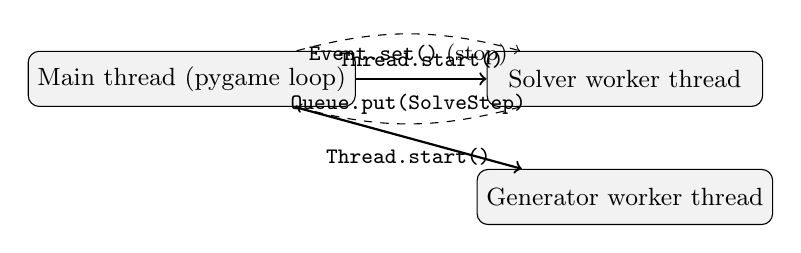
\begin{tikzpicture}[
    thread/.style={draw, fill=gray!10, rounded corners, minimum width=3.5cm,
                   minimum height=0.7cm, font=\small, text centered},
    msg/.style={->, dashed},
  ]
    \node[thread] (main)   at (0,0)    {Main thread (pygame loop)};
    \node[thread] (worker) at (5.5,0)  {Solver worker thread};
    \node[thread] (gen)    at (5.5,-1.5) {Generator worker thread};

    \draw[->, thick] (main) -- node[above, font=\footnotesize]
      {\texttt{Thread.start()}} (worker);
    \draw[->, thick] (main) -- node[below, font=\footnotesize]
      {\texttt{Thread.start()}} (gen);

    \draw[msg, bend left=15] (worker) to
      node[above, font=\footnotesize]{\texttt{Queue.put(SolveStep)}} (main);
    \draw[msg, bend left=15] (main) to
      node[below, font=\footnotesize]{\texttt{Event.set()} (stop)} (worker);
  \end{tikzpicture}
  \caption{Threading model.  The main thread owns all UI state; the worker
           thread communicates only via a thread-safe queue.}
  \label{fig:threading}
\end{figure}

The solver worker runs the selected algorithm and calls \texttt{on\_step} after
each node expansion.
\texttt{on\_step} decomposes bulk assignments into individual cell-fill steps
(so each cell appears one by one on screen), infers whether the step is a
backtrack by comparing filled-cell counts, and pushes a \texttt{SolveStep}
onto the queue.
A \texttt{threading.Event} (\texttt{stop\_event}) allows the main thread to
abort the worker cleanly: \texttt{on\_step} raises \texttt{StopIteration} if
the event is set, which the worker catches and exits silently.

The playback speed is controlled by a per-step \texttt{Event.wait(timeout=1/speed)}
inside \texttt{on\_step}: the worker thread \emph{itself} throttles its output
rate rather than the main thread buffering and rate-limiting separately.

The puzzle generator also runs in a daemon thread (no step-by-step output
needed) so the UI remains responsive during generation.

\subsubsection{Rendering (\texttt{ui})}

The renderer hierarchy follows the \emph{Composite} pattern:

\begin{description}
  \item[\texttt{CompositeRenderer}] Root renderer.
    Fills the background, fills the grid area, then delegates in draw order
    to \texttt{GridRenderer}, \texttt{ConstraintRenderer}, \texttt{HudRenderer}.

  \item[\texttt{GridRenderer}] Draws the $N \times N$ grid.
    Per-cell background colour is driven by \texttt{GameState} flags:
    given (grey), solver-assigned (blue), error (red), backtrack-flash (orange,
    fading over 0.5 s), shake-animation (invalid note attempt), selected (blue
    border).
    Values are drawn in the cell centre; pencil marks are drawn in sub-corners.

  \item[\texttt{ConstraintRenderer}] Draws the \texttt{<}/\texttt{>}/\texttt{\^}/\texttt{v}
    symbols in the pixel gaps between adjacent cells.

  \item[\texttt{HudRenderer}] Draws the right-hand side panel, divided into
    three sub-sections: Solver panel (play/pause/step/restart, speed, stats),
    Puzzle panel (load/generate with size and difficulty selectors),
    and Play panel (hint, undo, notes toggle).
\end{description}

All geometry is computed by \texttt{layout.py} based on fixed constants
(\texttt{SCREEN\_W=900}, \texttt{SCREEN\_H=680},
\texttt{SIDE\_PANEL\_W=260}).
\texttt{grid\_geometry(N)} scales the cell size to fit the grid area for any
$N \in \{4, \ldots, 9\}$.

\subsubsection{Input Handling (\texttt{app.InputHandler})}

\texttt{InputHandler.handle\_event()} dispatches pygame events to mode-specific
handlers:
\begin{itemize}
  \item Mouse clicks on the grid select cells; clicks on HUD buttons trigger
        mode switches, loads, generates, hints, undos, or solver controls.
  \item Number keys 1–$N$ enter values or toggle pencil marks depending on
        \texttt{notes\_mode}.
  \item \texttt{Backspace}/\texttt{Delete} clear the selected cell.
  \item \texttt{Ctrl+Z} calls \texttt{board.undo()}.
  \item Arrow keys advance the solver by one step in SOLVE mode.
\end{itemize}

% =============================================================================
\subsection{Entrypoint and CLI (\texttt{futoshiki\_vifeagent})}
\label{sec:layer_entry}

The top-level package \texttt{futoshiki\_vifeagent} exposes a single
\texttt{main()} that dispatches to three sub-commands:

\begin{description}
  \item[\texttt{python -m futoshiki\_vifeagent solver run --solver <key>}]
    Run the benchmark harness against the corpus.
  \item[\texttt{python -m futoshiki\_vifeagent solver generate}]
    Regenerate the benchmark corpus.
  \item[\texttt{python -m futoshiki\_vifeagent solver visualize}]
    Produce charts and \LaTeX\ tables from benchmark CSVs.
  \item[\texttt{python -m futoshiki\_vifeagent ui}]
    Launch the pygame application.
\end{description}

% =============================================================================
\subsection{Design Principles and Trade-offs}
\label{sec:design_principles}

\paragraph{Immutable problem vs.\ mutable state.}
\texttt{Puzzle} is the immutable problem definition; \texttt{Board} and
\texttt{SearchState} are mutable solving state.
This separation means solvers can safely share the same \texttt{Puzzle}
object across threads without copying constraint data.

\paragraph{Single state owner.}
All UI state lives in one \texttt{GameState} dataclass owned by the main
thread.
Worker threads communicate only through a \texttt{queue.Queue} and a
\texttt{threading.Event}.
This avoids locks on shared mutable state and makes the control flow easy to
follow.

\paragraph{Pluggable solvers via a single interface.}
\texttt{BaseSolver.solve(puzzle, on\_step)} is the only contract.
Adding a new solver requires only a new class and one entry in the
solver registry; no other code changes are needed.
The \texttt{on\_step} callback is optional so non-animated solvers (batch
mode) pay no overhead.

\paragraph{Separation of inference engines from domain knowledge.}
\texttt{ForwardChainingEngine} and \texttt{BackwardChainingEngine} have no
Futoshiki-specific logic: they operate on \texttt{HornClauseKnowledgeBase}
objects.
The KB construction is the domain-specific part; the inference machinery is
reusable.

\paragraph{Lazy constraint evaluation.}
AC-3 is not run unconditionally.
The A* engine runs basic singleton-fill by default; full AC-3 is only enabled
when the \texttt{AC3Propagator} is injected (used by \texttt{AStarSolver(h4)}).
This lets users compare the impact of arc consistency without changing the
algorithm.

\paragraph{Z3 for puzzle generation uniqueness.}
\texttt{FutoshikiGenerator} uses the Z3 SMT solver to verify that a candidate
puzzle has a unique solution.
This avoids implementing a second backtracking solver solely for the generator
and guarantees the uniqueness property without approximation.
